\newpage
\clearpage
\subsubsection{Estensione A: Annuncio in Sospeso}

In alcuni casi, un agente immobiliare potrebbe tentare di aggiungere un nuovo annuncio mentre ne ha già uno in sospeso. Per garantire un’esperienza utente fluida e prevenire la perdita accidentale di dati, il sistema mostra un pop-up che chiede esplicitamente se si desidera creare un nuovo annuncio o ripristinare quello precedente.

\subsubsection{Gestione del Pop-up e Scelta dell’Utente}
All’azione di aggiunta di un nuovo annuncio con un annuncio incompleto in sospeso, viene visualizzato un messaggio di conferma con due opzioni:
\begin{itemize}
    \item \textbf{Crea un nuovo annuncio}: l’utente sceglie di avviare un nuovo processo di inserimento. Il sistema informa chiaramente che i dati dell’annuncio precedente andranno persi.
    \item \textbf{Ripristina l’annuncio precedente}: il sistema recupera i dati salvati localmente e ripristina il modulo alla condizione precedente.
\end{itemize}

Questa decisione è fondamentale per garantire il controllo dell’utente sull’operazione e per evitare errori involontari che potrebbero compromettere l’inserimento dell’annuncio.

\subsubsection{Estensione A: Creazione di un Nuovo Annuncio}
Se l’utente seleziona \textbf{Crea un nuovo annuncio}, il sistema mostra un messaggio di conferma che avvisa della perdita definitiva dei dati precedentemente salvati. Questa scelta progettuale si basa sul principio della \textbf{prevenzione degli errori} \cite{nielsen1995}, poiché aiuta a evitare cancellazioni accidentali e garantisce una maggiore consapevolezza dell’azione intrapresa.

Il messaggio di conferma include due pulsanti:
\begin{itemize}
    \item \textbf{Annulla}: consente di tornare indietro senza perdere i dati in sospeso.
    \item \textbf{Procedi}: conferma l’azione e avvia un nuovo annuncio.
\end{itemize}


\begin{figure}[ht]
    \centering
    \begin{tikzpicture}[node distance=1.5cm and 1cm, auto]
        % Nodo per immagine 1 con didascalia sotto
        \node (img1) {
            \begin{tabular}{c}
                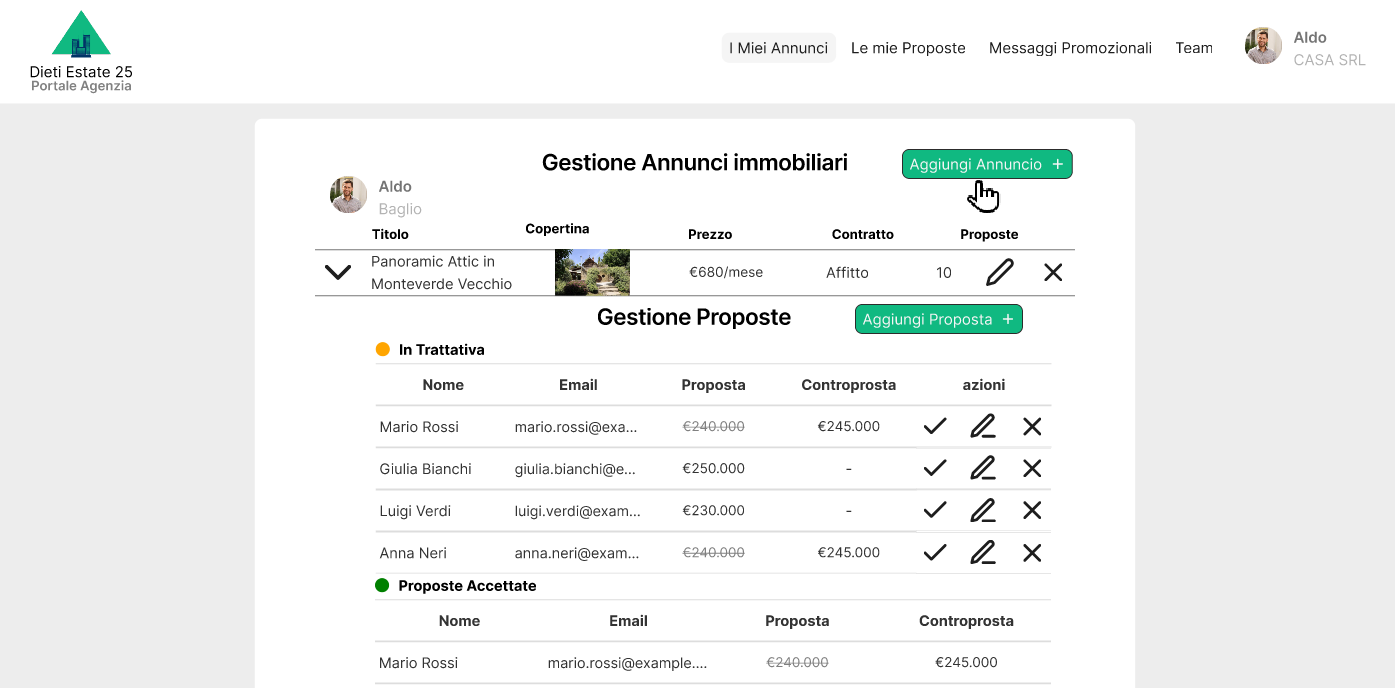
\includegraphics[width=0.7\textwidth]{Immagini/Mockup/aggiungi annuncio/estensione A/step1.png} \\
                click nuovo annuncio
            \end{tabular}
        };
        
        % Nodo per immagine 2 con didascalia sotto, posizionato a destra di img1
        \node (img2) [below=of img1] {
            \begin{tabular}{c}
                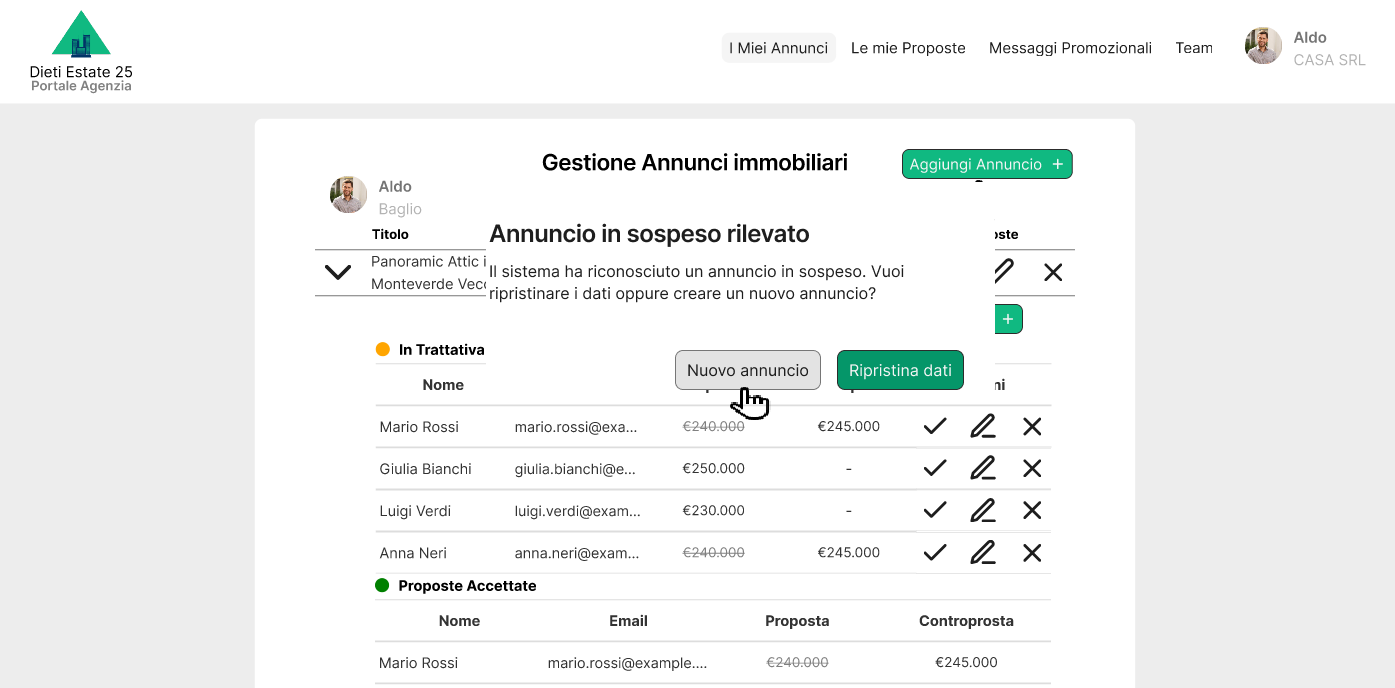
\includegraphics[width=0.7\textwidth]{Immagini/Mockup/aggiungi annuncio/estensione A/step2.png} \\
                Cockburn: extension A.2/A.3/A.4
            \end{tabular}
        };
        
        % Nodo per immagine 3 con didascalia sotto, posizionato sotto img2
        \node (img3) [below=of img2] {
            \begin{tabular}{c}
                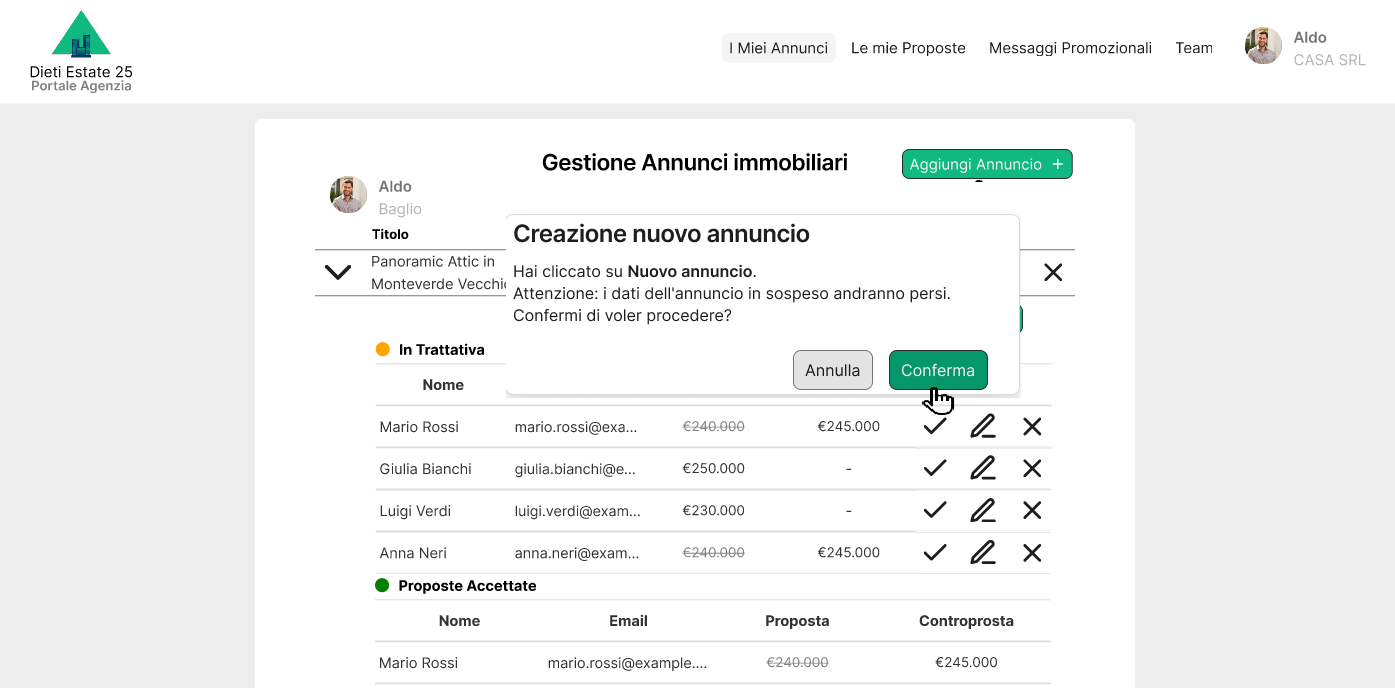
\includegraphics[width=0.7\textwidth]{Immagini/Mockup/aggiungi annuncio/estensione A/step3.png} \\
                Cockburn: extension A.6
            \end{tabular}
        };
        
        % Disegna le frecce
        \draw[->, thick] (img1) -- (img2);
        \draw[->, thick] (img2) -- (img3);
      
    \end{tikzpicture}
    \caption{Mockup: estensione A della tabella di Cockburn del caso d'uso nuovo annuncio}
    \label{fig:tikz_flow}
\end{figure}

\newpage

